\documentclass[times,11pt]{report}
\usepackage{fullpage}
\usepackage{graphicx}
\usepackage[colorlinks=true,linkcolor=black]{hyperref}
\usepackage{hyperref}
\usepackage{mathptmx} % - sets \rmdefault to 'ptm', i.e. times
\renewcommand{\familydefault}{ptm} % using \rmdefault here doesn't work
\begin{document}
\title{Savant Genome Browser: Plugin Development Guide}
%\author{Marc Fiume \& Eric Smith}
\maketitle

\setlength{\parindent}{0pt} 
\setlength{\parskip}{2ex}

Authors: Marc Fiume \& Eric Smith\\
Contact: savant@cs.toronto.edu \\
Website: http://savantbrowser.com \\
\\
This document applies to Savant SDK version 2.0.0\\

\newpage

\tableofcontents

\newpage

\chapter{Introduction}

Savant is unique in the Genome Browser arena in that it was designed to be extensible through a rich plugin framework, which allows developers to provide functionality in addition to what is provided with the standard distribution.

A wide range of Savant plugins have already been written.  GUI plugins, like the Amino Acid plugin and the SNP Finder, enhance the visualisation of data within Savant  (see Chapter~\ref{SampleGUIPlugin}).  DataSource plugins, like the SQL plugin and the UCSC plugin, extend Savant by providing access to new sources of data  (Chapter~\ref{SampleDataSourcePlugin}).  Tool plugins, like the GATK tool, extend Savant by providing integrated access to third-party analytical tools (Chapter~\ref{SampleToolPlugin}).

\chapter{Tutorial: Developing a Savant Plugin}
In this tutorial, we describe the steps used to create the Savant Amino plugin using the demo project included in the Savant SDK as a template.

\section{The Amino Plugin}
The Savant Amino plugin was designed to demonstrate just some aspects of the API: in particular, accessing basic information about tracks and rendering it within Savant. It does not cover much of what is offered through the API (for example, creating custom data-sources or visualisations). Most importantly, this tutorial was designed to help you create a foundation for your own plugin project.

\begin{figure}[h]
\begin{center}

\includegraphics[type=png,ext=.png,read=.png,width=15cm]{images/AminoPlugin}
\end{center}
\end{figure}

\section{Prerequisites}
\begin{itemize}
	\item JDK
	\item NetBeans\\
		Note: for this tutorial, it is recommended to download the Netbeans + JDK Bundle from \href{http://www.oracle.com/technetwork/java/javase/downloads}{oracle.com}.
	\item Savant SDK
\end{itemize}

\section{Setting Up the NetBeans Project}
\subsection*{1. Set up NetBeans and the JDK}
Download NetBeans and the JDK and install them. For simplicity it is recommended to download the bundle, but you can certainly download and install them independently if you wish.
\subsection*{2. Set up the Savant SDK}
Download the Savant SDK, listed above, and unzip it. The SDK contains the following components:
\begin{itemize}
	\item api -- documentation of the Savant code
	\item dev -- development files
	\item samples -- sample projects
	\item this file
\end{itemize}
For this tutorial, we will refer to the dev folder in the SDK as dev/.
\subsection*{3. Open the Demo Project}
Open NetBeans. Open the project in dev/savant.demo.

\begin{figure}[h]
\begin{center}
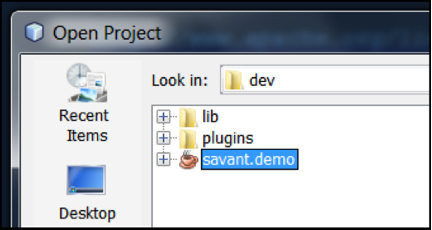
\includegraphics[type=png,ext=.png,read=.png,width=9cm]{images/OpenProject}
\end{center}
\end{figure}
\newpage
The ``Project'' and ``Files'' views should look something like this:
\begin{figure}[h]
\begin{center}
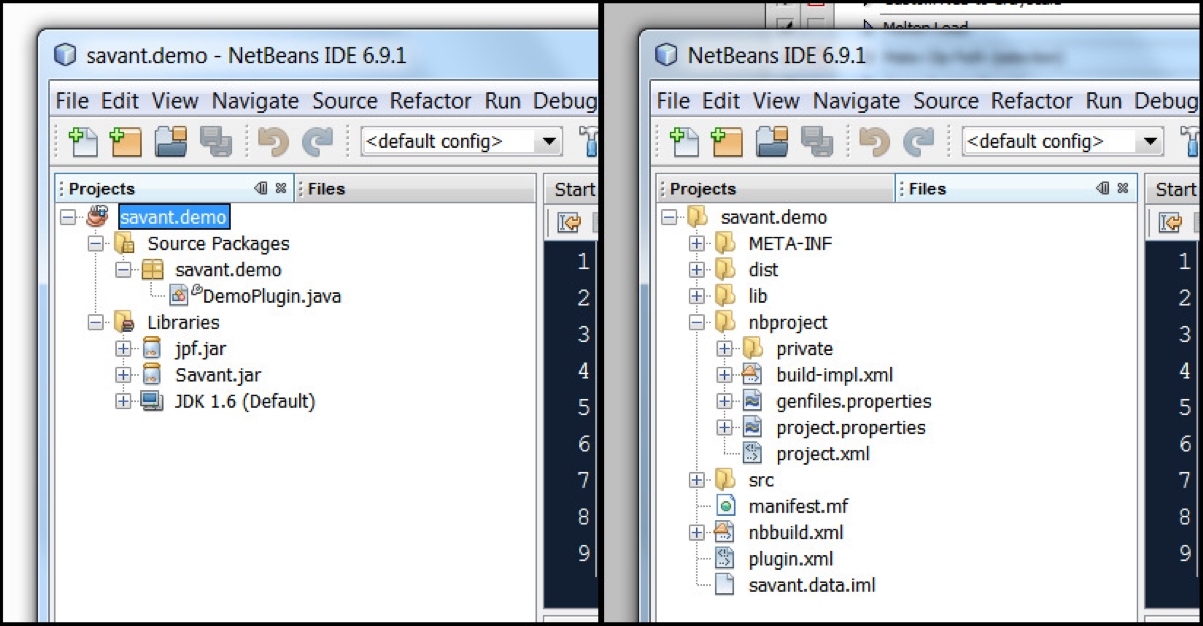
\includegraphics[type=png,ext=.png,read=.png,width=15cm]{images/ProjectAndFiles}
\end{center}
\end{figure}

\subsection*{Description of Important Project Files}
\begin{itemize}
	\item Project View
	\begin{itemize}
		\item Source Packages -- contains implementation of this plugin
		\begin{itemize}
			\item Main package (savant.demo) -- contains the main class of the plugin
			\item Main class (DemoPlugin.java) -- the class which implements the Savant Plugin interface
		\end{itemize}
		\item Libraries -- contains links to external code packages
		\begin{itemize}
			\item Savant.jar -- Savant API, required for accessing Savant functions
		\end{itemize}
	\end{itemize}
	\item Files View
	\begin{itemize}
		\item lib/ -- contains additional libraries used by this plugin
		\item nbproject/project.properties -- contains NetBeans project properties
		\item nbbuild.xml -- contains Ant instructions for building the project
		\item plugin.xml -- contains information about the plugin and how to run it
	\end{itemize}
\end{itemize}

\section{Editing the Demo Project}
You will need to know the following properties of your plugin:
\begin{itemize}
	\item \textit{NAME} -- the name of the plugin.
	\item \textit{VERSION} -- the version of the plugin. In Savant we use the following scheme for version numbers [major version] . [minor version] . [bug fix / build number].
	\item \textit{PACKAGE} -- the main package of the plugin (which contains the main class).
	\item \textit{CLASS} -- the main class of the plugin.
\end{itemize}
In this example, \textit{NAME}~= ``Amino Plugin'', \textit{VERSION}~= ``1.0.0'', \textit{PACKAGE}~= ``savant.amino'', and \textit{CLASS}~= ``AminoPlugin''.

\subsection*{1. Copy the Demo Project}
Right-click the savant.demo project icon (looks like a coffee cup) and choose ``Copy\ldots''. The copy dialog will be presented. In the Project Name field, enter \textit{PACKAGE}. Click the ``Copy'' button.
\begin{figure}[h!]
\begin{center}
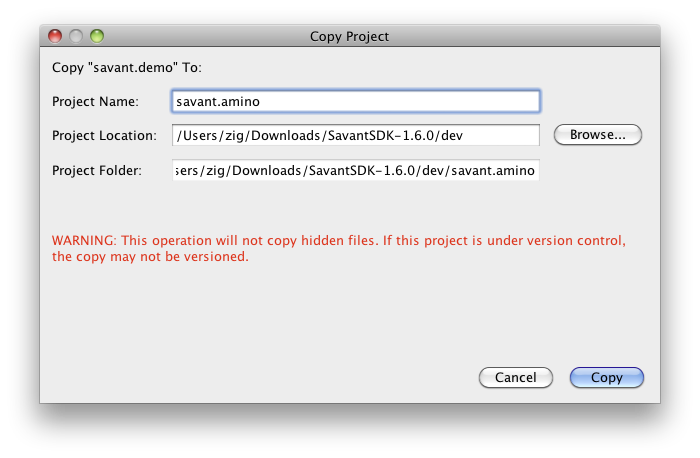
\includegraphics[type=png,ext=.png,read=.png,width=11cm]{images/CopyProject}
\end{center}
\end{figure}

This will create a copy of the demo project which we will now edit to create a new plugin.
\subsection*{2. Rename the main package}
Right-click the savant.demo package icon (looks like a cardboard box) and choose ``Refactor \textgreater~Rename\ldots''. In the New Name field, enter \textit{PACKAGE}. Click the ``Refactor'' button.
\begin{figure}[h!]
\begin{center}
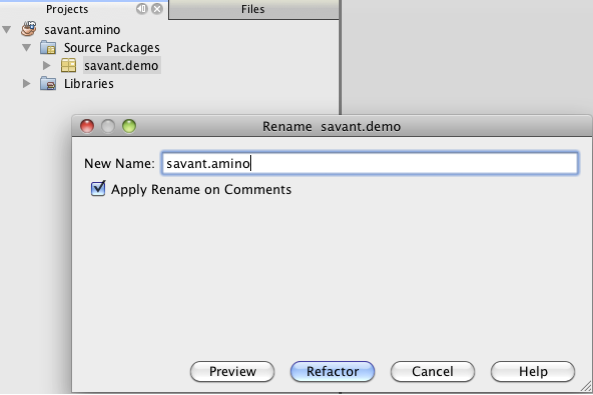
\includegraphics[type=png,ext=.png,read=.png,width=10cm]{images/RenamePackage}
\end{center}
\end{figure}

\subsection*{3. Rename the main class}
Right-click the DemoPlugin.java icon and choose ``Refactor \textgreater~Rename\ldots''. In the New Name field, enter \textit{CLASS}. Click the ``Refactor'' button.

\subsection*{4. Change the plugin name}
Double-click the \textit{CLASS}.java file (formerly DemoPlugin.java) to open it in the Editor. Change the {\tt getTitle()} function to return ``\textit{NAME}''.
\begin{figure}[h!]
\begin{center}
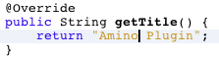
\includegraphics[type=png,ext=.png,read=.png]{images/RenamePlugin}
\end{center}
\end{figure}

\subsection*{5. Edit the plugin properties}
Switch to the ``Files'' view (the tab beside the ``Projects'' tab). Expand the new project. Double-click the plugin.xml  file to open it in the editor. There are four places that need to be edited in this file, denoted in red boxes in the following figure:
\begin{figure}[h!]
\begin{center}

\includegraphics[type=png,ext=.png,read=.png,width=16cm]{images/PluginXML}
\end{center}
\end{figure}

Here is how the file will be changed in the savant.amino example:
\begin{figure}[h!]
\begin{center}

\includegraphics[type=png,ext=.png,read=.png,width=16cm]{images/PluginXML2}
\end{center}
\end{figure}

\subsection*{6. Change the project name}
Open the nbbuild.xml file in the editor (it's in the same directory as plugin.xml). Change the name attribute of the project to \textit{PACKAGE}.
\begin{figure}[h!]
\begin{center}
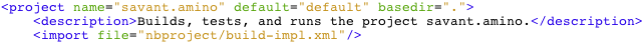
\includegraphics[type=png,ext=.png,read=.png,width=16cm]{images/RenameProject}
\end{center}
\end{figure}

At this point, we have created an independent plugin project which can be built and loaded into Savant. It is a good idea to try to do so now. See the section on building plugins (\S\ref{BuildingPlugins}).

\section{Code Away!}
You now have an independent plugin project as a foundation for your own plugin. You have two main tasks, outlined below. If you are following the savant.amino tutorial, you should download the complete savant.amino NetBeans Project to a separate location and copy the Java files in the dev/src directory of that package to the dev/src directory of your NetBeans project (overwriting AminoPlugin.java).

In general, the remaining tasks are:

\subsection*{1. Implementing the {\tt init()} function}
The {\tt init()} function is called immediately when the plugin is loaded as Savant starts. The init function is responsible for initializing (among other things) the graphical components of the plugin (e.g. buttons, menus, etc.). The graphical "canvas" for plugins is a JPanel provided as an argument to the {\tt init()} function. For help with JPanel and other Swing components visit \href{http://download.oracle.com/javase/tutorial/uiswing}{http://download.oracle.com/javase/tutorial/uiswing}.

\subsection*{2. Implementing the rest of your plugin}
Go nuts, you are free to do whatever you like in your plugin!

\subsection*{Suggested guidelines:}
\subsubsection{Thread long running tasks}
Your plugin will run in the main Savant thread unless you tell it to do otherwise. This means that if your plugin does something which takes a long time (e.g. downloads files, performs a long computation, etc.) it will lock up the main thread until it has finished. Please perform such tasks in a separate thread.\\

\subsubsection{Try to stick to what's in the Savant API packages}
The {\tt savant.api.adapter} and {\tt savant.api.util} packages contains classes and methods which the Savant development team considers useful for developers to have. It is possible a developer requires some more functionality that can be found by getting access to a Savant instance. Please notify us of these situations so that we can consciously include such functionality in subsequent versions of the API, otherwise there is a risk that this functionality will be destroyed (since we're not expecting anyone to be using it directly) and your plugin will no longer work.

\section{Submit Your Plugin}
We strongly encourage you to submit all your developed Savant plugins to us, so that we can make them directly available to all Savant users through the Savant Plugin Repository. This is both a great way to promote your own work while encouraging more users and developers to join the Savant Community! You can submit your plugins to us through our plugin submission form: \href{http://savantbrowser.com/plugins.php\#submit}{http://savantbrowser.com/plugins.php\#submit}.

\chapter{Plugin Development Tips and Tricks}
\section{Building and Testing Plugins}
\label{BuildingPlugins}
To build your plugin, right-click the plugin project icon (the coffee cup) and choose ``Build''. NetBeans should output something like this:
 
\begin{figure}[h!]
\begin{center}
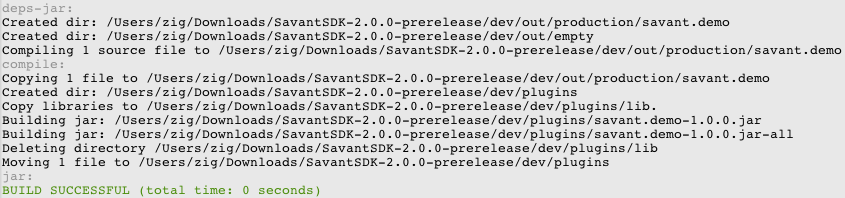
\includegraphics[type=png,ext=.png,read=.png,width=15cm]{images/BuildOutput}
\end{center}
\end{figure}

What's important is that it builds successfully. Look in the dev/plugins directory. You should see a .jar file corresponding to your plugin (in the savant.amino example, it is savant.amino-1.0.0.jar).

Now that you've ensured that the plugin was built, you can test out the plugin by running the provided dev/testPlugins.sh script or by running the Savant.jar otherwise (e.g. in Windows, you can just double-click Savant.jar).
\section{Including Other Libraries}
You may include additional libraries in your plugin. To do so:
\begin{enumerate}
\item Place the jar file for the external library in the dev/lib folder.
\item In your NetBeans project, right-click ``Libraries'', then choose ``Add JAR/Folder\ldots'', then find the jar file and click ``Open''.
\item Open the nbbuild.xml file in the ``Files'' view in NetBeans, and add a new {\tt zipfileset} entry under the previous {\tt zipfileset} entry (near the bottom of the file) for your jar file:
\begin{figure}[h!]
\begin{center}
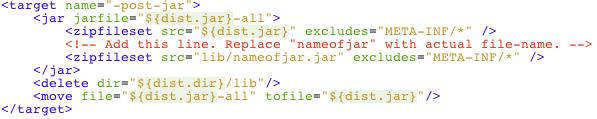
\includegraphics[type=png,ext=.png,read=.png,width=15cm]{images/ZipFileSet}
\end{center}
\end{figure}
\end{enumerate}

\chapter{Sample GUI Plugin: savant.amino}
\label{SampleGUIPlugin}
In the samples/savant.amino directory of the SDK download, you will find the completed savant.amino plugin.  The code is divided into three files: AminoPlugin.java, AminoAcid.java, and AminoCanvas.java.

The Amino Acid plugin is an example of a GUI plugin which renders extra information in a layer on top of one of the existing tracks.

\section{AminoPlugin.java}
The actual class which implements the Savant plugin.  Since this is a GUI plugin, the class it extends is {\tt SavantPanelPlugin}.  The {\tt AminoPlugin} class has only three methods of note:  {\tt init()}, {\tt getTitle()}, and {\tt getAlpha()}. The first two of these methods are required by the {\tt SavantPanelPlugin} interface.

\subsection{\tt AminoPlugin.init()}
Initialises the plugin's interface panel.  This panel is what the user will see upon selecting the plugin's tab at the bottom of the Savant window.  What the plugin puts in this panel is entirely up to you.  For some plugins, like the built-in Data Table plugin, the panel is the essential part of the plugin, for others the panel just provides a way of configuring the plugin's settings.  Since the savant.amino plugin has no real settings to configure, the panel contains only a legend describing the colour scheme used by the plugin.

The {\tt init()} function also gives the plugin an opportunity to register listeners for Savant events it might be interested in.  In this case, the savant.amino plugin listens for {\tt TrackEvent}s and {\tt LocationChangedEvent}s.  The former gives the plugin a chance to create an {\tt AminoCanvas} on which to draw the track's amino acids; the latter lets the plugin know when the layer canvas needs to be repainted.

\subsection{\tt AminoPlugin.getTitle()}
This required method provides the title for the plugin's tab in the Savant user interface.

\subsection{\tt AminoPlugin.getAlpha()}
An example of how a plugin can access persistent settings stored in the savant.settings file.  As an exercise, you can add a {\tt JSlider} to the plugin's panel and use {\tt SettingsUtils.setInt()} to save the value programmatically.  For the time being, changing the settings will require adding a line like ``savant.amino.ALPHA=40'' to your \textasciitilde/.savant/savant.settings file.

\section{AminoAcid.java}
This enum defines the constants associated with each amino acid, and sets up a lookup table.  The colour scheme is taken from RasMol, which assigns colours according to traditional amino acid properties (e.g. aspartic acid and glutamic acid are acidic and coloured red, while arginine, histidine, and lysine are basic and coloured in bluish shades).

\section{AminoCanvas.java}
This class does the work of actually drawing the amino acids.  The plugin creates an {\tt AminoCanvas} when it receives a {\tt TrackEvent.Type.ADDED} event from Savant, and adds the newly-created canvas to the track's layer-canvas.  Since the {\tt AminoCanvas} will be drawn on top of the track itself, it calls {\tt setOpaque(false)} to ensure that it doesn't completely obscure the track.

The plugin converts between base positions and pixel values using the {\tt TrackAdapter}'s {\tt transformXPos()} method. Information about where the starts and ends of coding regions is retrieved using the track's {\tt getDataInRange()} method, which returns a list of records.  In this case, since the plugin only attaches an {\tt AminoCanvas} to tracks with data-format {\tt RICH\textunderscore INTERVAL}, we can assume that it's safe to cast these records to {\tt RichIntervalRecord}.

The actual sequence data is retrieved using the {\tt GenomeAdapter} class.  The rest of the plugin's logic is devoted to figuring out where the codons start and end.

\chapter{Sample DataSource Plugin: savant.diff}
\label{SampleDataSourcePlugin}
The savant.diff plugin is intended to demonstrate how to write a data-source plugin.  The data-source plugins most familiar to Savant users are probably the UCSC and SQL plugins, which let Savant display data retrieved from a relational database.  For the purposes of the SDK, we will present a much simpler plugin, which calculates the difference between two continuous tracks and displays the result as a third such track.

\section{DiffPlugin.java}
The actual class which implements the Savant plugin.  Since this is a data-source plugin, it is derived from {\tt SavantDataSourcePlugin}.  The {\tt init()} and {\tt getTitle()} methods are required by the plugin interface, but don't do anything particularly interesting.  The actual work is done in the two {\tt getDataSource()} methods.

\subsection{\tt DiffPlugin.getDataSource()}
The niladic version of {\tt getDataSource()} is called by Savant when the user chooses the \textit{Load Track from Other DataSource} option from the \textit{File} menu.  In the case of the Diff plugin, this just presents a dialog to let the user select which two continuous tracks will serve as inputs for the plugin.

More elaborate plugins, such as the UCSC plugin, use this method as an opportunity to log into a database and configure a session.  Regardless of the complexity of this configuration process, the results should all be distilled into a single URI which contains sufficient information to save and restore the session.  In the case of the Diff plugin this URI consists of the scheme {\tt diff://} followed by the URIs for the two input tracks, enclosed in brackets and separated by a semicolon.  Together this provides enough information for the plugin to reconstitute the Diff track later.

\subsection{\tt DiffPlugin.getDataSource(URI)}
This version of the {\tt getDataSource()} method is used when opening a project or using the \textit{Recent Tracks} menu.  It takes the {\tt diff://} URI and determines which two tracks to use as inputs.  If the Diff plugin were production code, it would include logic to open the input tracks if they were not already loaded.  However, since this plugin is just intended as sample code, that extra logic has been omitted for the sake of clarity.

\section{SourceDialog.java}
Provides a simple user interface that lets the user select which tracks to use as inputs for the Diff track.  The track lists are populated using {\tt TrackUtils.getTracks(DataFormat.CONTINUOUS)}, which provides an array of all loaded continuous tracks, including both ordinary continuous tracks as well as coverage tracks.

\section{DiffDataSource.java}
This class provides the plugin's implementation of the {\tt DataSourceAdapter} interface.  Savant uses parameterised types for its data-sources, so the actual interface implemented is {\tt DataSourceAdapter<ContinuousRecord>}.  The {\tt ContinuousRecord} interface consists of just a position, a reference (i.e. chromosome), and a floating-point value.

The {\tt DataSourceAdapter} interface requires nine methods to be implemented, but seven of them are trivial.  The {\tt getDataFormat()} and {\tt getColumnNames()} methods just return constants which are appropriate for continuous tracks.  The {\tt getURI()} method returns the URI which was set by the track's constructor.  For want of anything better to return, the plugin just returns the track's URI as the value for {\tt getName()}.  The {\tt loadDictionary()} and {\tt lookup()} methods are intended for tracks which have named features (e.g. gene tracks); for a continuous track these methods can just be stubs.  Similarly, the Diff plugin has no cleanup to perform, so the {\tt close()} method can also just be a stub.

\subsection{\tt DiffDataSource.getReferenceNames()}
The {\tt getReferenceNames()} method is used by Savant to determine which references a track has data for.  For a Diff track, this is essentially the intersection of the references for its two inputs. In practice, some tracks store references as ``chr1'', ``chr2'', etc., while others use ``1'', ``2'', which means that {\tt getReferenceNames()} needs to have a bit of extra logic to homogenise these two representations.

\subsection{\tt DiffDataSource.getRecords()}
The key method of any data-source is {\tt getRecords()}.  Savant passes the plugin a reference, a range, and a resolution, and the data-source is supposed to return a list of data records, ordered by ascending position.  In the case of the Diff plugin, this just amounts to calling {\tt getRecords()} for the two input tracks and calculating the difference between the values at each position.  This is complicated somewhat by the fact that there is no guarantee that the input data-sources will return a data-record for every position (particularly at lower resolutions), hence the need for the {\tt interpolate()} method.

\chapter{Sample Tool Plugin: srma.xml}
\label{SampleToolPlugin}
Tool plugins are a new variety of plugins which was introduced in Savant 2.  They provide a way to wrap an external application so that it can be invoked from within Savant.

A tool plugin is defined by an XML file which describes how to invoke the external application, how to specify its arguments, and how to interpret its output.  The format of this XML file is derived from the plugin.xml file used for other Savant plugins.  Other Savant plugins embed the plugin.xml file inside a JAR file, but tool plugins consist solely of the bare XML file.

To the end-user, a tool plugin looks much like an ordinary GUI plugin.  A tool has a user-interface which is presented in a tab at the lower left of the Savant window.  The various command-line arguments can be configured using that user-interface.  Clicking the ``Execute'' button will launch the external application, and the application's progress and status will be displayed in the tool's panel.

The actual installation of the external application lies outside the scope of this document.  The sample tool plugin included with the SDK executes SRMA (\href{http://dx.doi.org/10.1186/gb-2010-11-10-r99}{Homer and Nelson 2010}), which happens to be a Java application.  However, a tool plugin can equally well be used to invoke a platform-specific binary.

\section{{\tt\textless plugin\textgreater} Element}
The top-level element of a tool plugin's XML file is the {\tt\textless plugin\textgreater} element.  Like the {\tt\textless plugin\textgreater} element of a plugin.xml file, this element has attributes for {\tt id}, {\tt version}, {\tt class}, {\tt sdk-version}, and {\tt name}.  The only special requirement for a tool plugin is that the {\tt class} attribute be {\tt savant.plugin.Tool}.

\begin{figure}[h!]
\begin{center}
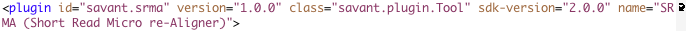
\includegraphics[type=png,ext=.png,read=.png,width=15cm]{images/ToolPluginXML}
\end{center}
\end{figure}

\section{{\tt\textless tool\textgreater} Element}
The tool's XML file should contain a single {\tt\textless tool\textgreater} element, defining the command-line which will be executed to invoke the tool.

In the case of the SRMA sample, the command line launches Java to invoke the srma JAR file.  Here, the actual srma-0.1.15.jar\footnote{This JAR file is not included as part of the Savant SDK.  It should be downloaded from \href{http://sourceforge.net/projects/srma/files}{http://sourceforge.net/projects/srma/files} and copied to your \textasciitilde/.savant/plugins directory (savant\textbackslash plugins on Windows).} file is expected to be in the Savant plugins directory (\textasciitilde/.savant/plugins).  Any invariant command-line options can also be specified in the {\tt\textless tool\textgreater} element.

\section{{\tt\textless arg\textgreater} Elements}
Following the {\tt\textless tool\textgreater} element can be any number of {\tt\textless arg\textgreater} elements.  Each {\tt\textless arg\textgreater} tag describes a single command-line argument.

The {\tt flag} attribute indicates the text of the flag as it will be inserted onto the external application's command-line.  To make it clearer, the actual command-line is displayed at the top of the plugin's panel as the user manipulates the user-interface.

The user-interface is generated programmatically using the {\tt name} and {\tt type} attributes.  The {\tt name} provides a user-friendly name which will be used when presenting the argument in the user-interface.  The argument's appearance in the user-interface is controlled by the {\tt type} attribute, as described in the following table.

\begin{table}[h!]
\begin{tabular}{|l p{10cm}|}
\hline
Type & Presentation\\
\hline\hline
{\tt BAM\textunderscore INPUT\textunderscore FILE} & Menu listing all open alignment tracks\\
{\tt FASTA\textunderscore INPUT\textunderscore FILE} & Menu listing all open sequence tracks\\
{\tt OUTPUT\textunderscore FILE} & Text-field \\
{\tt RANGE} & Savant-style range specification (e.g. ``chr1:1-1000'')\\
{\tt BOOL} & Check-box\\
{\tt INT} & Text-field to enter integer value\\
{\tt FLOAT} & Text-field to enter floating-point number\\
{\tt LIST} & Uses {\tt\textless arg\textgreater}'s {\tt choices} attribute to populate a menu.  Choices are expected to be comma-separated.\\
{\tt MULTI} & Uses {\tt choices} attribute to populate a grid of check-boxes.  Allows user to select multiple options.\\
\hline
\end{tabular}
\end{table}

As it happens, there are no {\tt type="MULTI"} arguments for the SRMA sample, but here is an example of one from the GATK tool, which allows multiple occurrences of the \textit{-G} argument to appear on its command-line:

\begin{figure}[h!]
\begin{center}

\includegraphics[type=png,ext=.png,read=.png,width=15cm]{images/MultiArg}
\end{center}
\end{figure}

In addition to the required attributes described so far, the {\tt\textless arg\textgreater} element has two optional attributes:  {\tt required} and {\tt default}.  Most arguments are presented with a check-box next to them which lets the user control whether they should appear on the command-line, but if an argument has the {\tt required="true"} attribute, a value must be specified.

\section{{\tt\textless progress\textgreater} and {\tt\textless error\textgreater} Elements}
When executing an external application as a plugin tool, Savant reads the application's standard output and standard error streams, in order to display it in the plugin's panel.  In many cases, this output can also be parsed to determine the progress and status of the external application.  Knowing the expected pattern of output, Savant can optionally apply a regular expression to extract that information.  The example below shows the regular expressions which are used by the GATK tool plugin.

\begin{figure}[h!]
\begin{center}
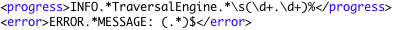
\includegraphics[type=png,ext=.png,read=.png]{images/RegExps}
\end{center}
\end{figure}

\end{document}
